\documentclass{beamer}
\usepackage[utf8]{inputenc}
\usepackage{amsmath, pdfpages, pdflscape, lscape, color, listings, hyperref, amssymb, graphicx,textcomp,varioref, afterpage, subcaption, float, bm, tikz} 

\global
\newcommand{\Fig}[1]{Figure \ref{#1}}
\newcommand{\fig}[1]{figure \ref{#1}}
\newcommand{\tab}[1]{table \ref{#1}}
\newcommand{\eq}[1]{equation \ref{#1}}
\newcommand{\Eq}[1]{Equation \ref{#1}}
\newcommand{\alg}[1]{algorithm \ref{#1}}
\newcommand{\Alg}[1]{Algorithm \ref{#1}}
\newcommand{\chp}[1]{chapter  \ref{#1}}
\newcommand{\Chp}[1]{Chapter  \ref{#1}}
\newcommand{\e}[1]{\cdot 10^{#1}}
\newcommand{\h}{\hbar}
\newcommand{\der}[2]{\frac{\partial #1}{\partial #2}}
\newcommand{\dder}[2]{\frac{\partial^2 #1}{\partial #2^2}}
\newcommand{\p}{\boldsymbol{P}}
\newcommand{\q}{\boldsymbol{q}}
\newcommand{\norm}[1]{\left\lVert#1\right\rVert_{\!Q}}
\newcommand{\inner}[1]{\left\langle#1\right\rangle_{\!Q}}
\newcommand{\coef}[2]{\frac{\inner{#1,#2}}{\norm{#2}^2}}

\DeclareMathOperator*{\argmin}{argmin}
\DeclareMathOperator*{\argmax}{argmax}

\newcommand{\E}[1]{\mbox{E}\!\left(#1\right)}
\newcommand{\Var}[1]{\mbox{Var}\!\left(#1\right)}
\newcommand{\Cov}[1]{\mbox{Cov}\!\left(#1\right)}

\newenvironment{test}[1]
{
 \usebackgroundtemplate{}
 \color{gray!30!black}
   \begin{tikzpicture}[remember picture, overlay]
     \node[anchor = center, opacity=.25] (image) at (current page.center) {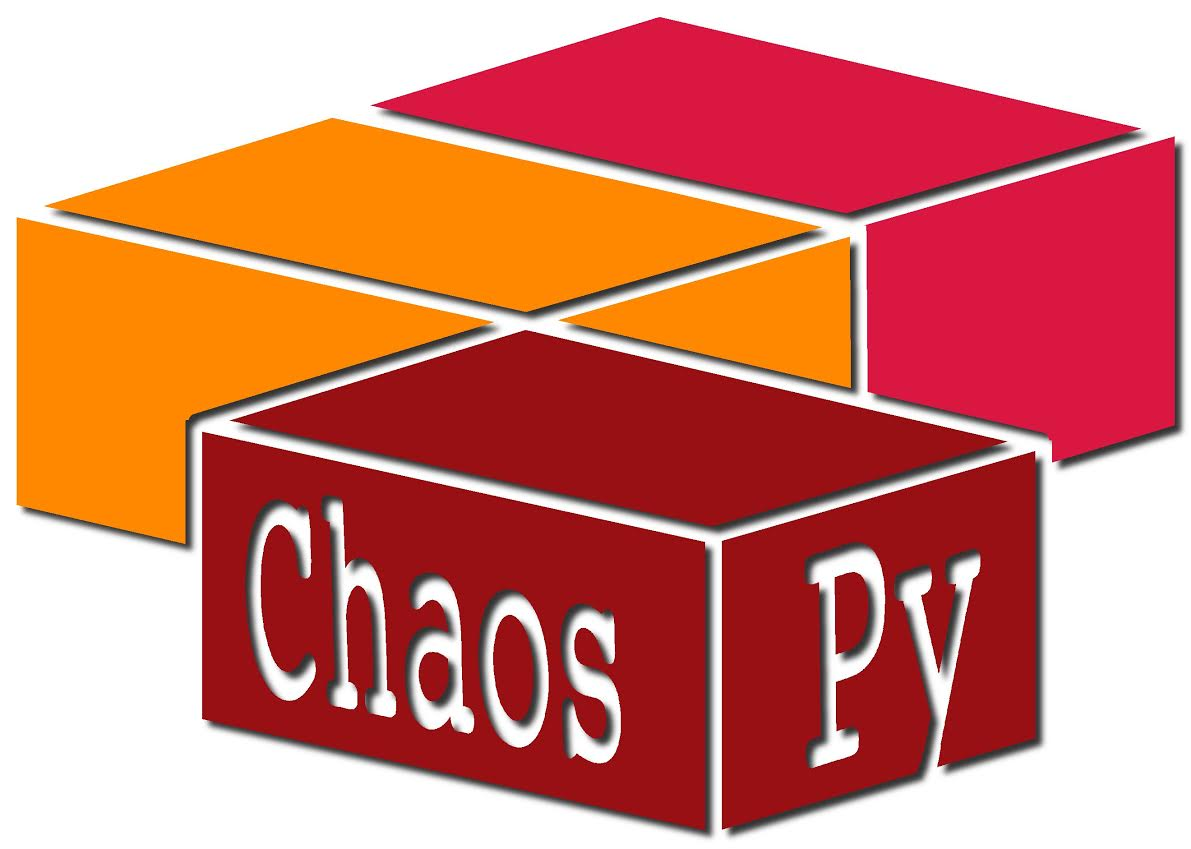
\includegraphics[scale=0.25]{chaospy_logo.jpg}};
   \end{tikzpicture}
 \begin{frame}[fragile,environment=chaospy]
   
}
{
 \end{frame}
}


\newenvironment{chaospy}[1]
{\color{gray!30!black}
     \color{gray!30!black}
     \usebackgroundtemplate{
   \begin{tikzpicture}[remember picture, overlay]
     \node[anchor = center, opacity=.25] (image) at (current page.center) {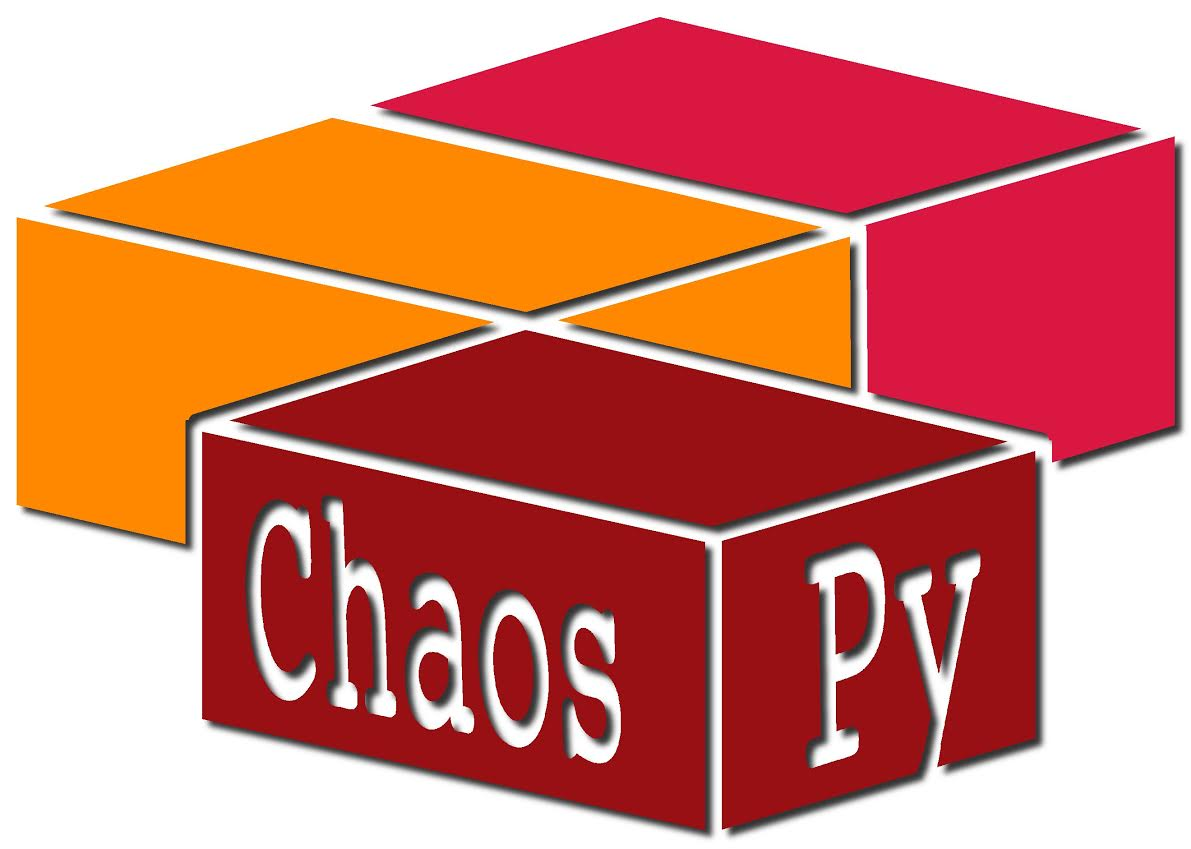
\includegraphics[scale=0.25]{chaospy_logo.jpg}};
   \end{tikzpicture}}
     \begin{frame}[fragile,environment=chaospy]
    \frametitle{{#1}}}
{\end{frame}}


\definecolor{keywords}{RGB}{255,0,90}
\definecolor{comments}{RGB}{0,0,113}
\definecolor{red}{RGB}{160,0,0}
\definecolor{green}{RGB}{0,150,0}
 
 
 \lstset{
escapeinside=||
}

 
\usetheme{kalkulo}

\graphicspath{{./figures/}}


\title{Polynomial chaos expansions part I: Method Introduction}
\author{Jonathan Feinberg and Simen Tennøe}


\begin{document}


\begin{frame}
  \maketitle
\end{frame}

\begin{frame}[fragile]{Lecture will include many examples using the
    Chaospy software}
  \begin{center}
     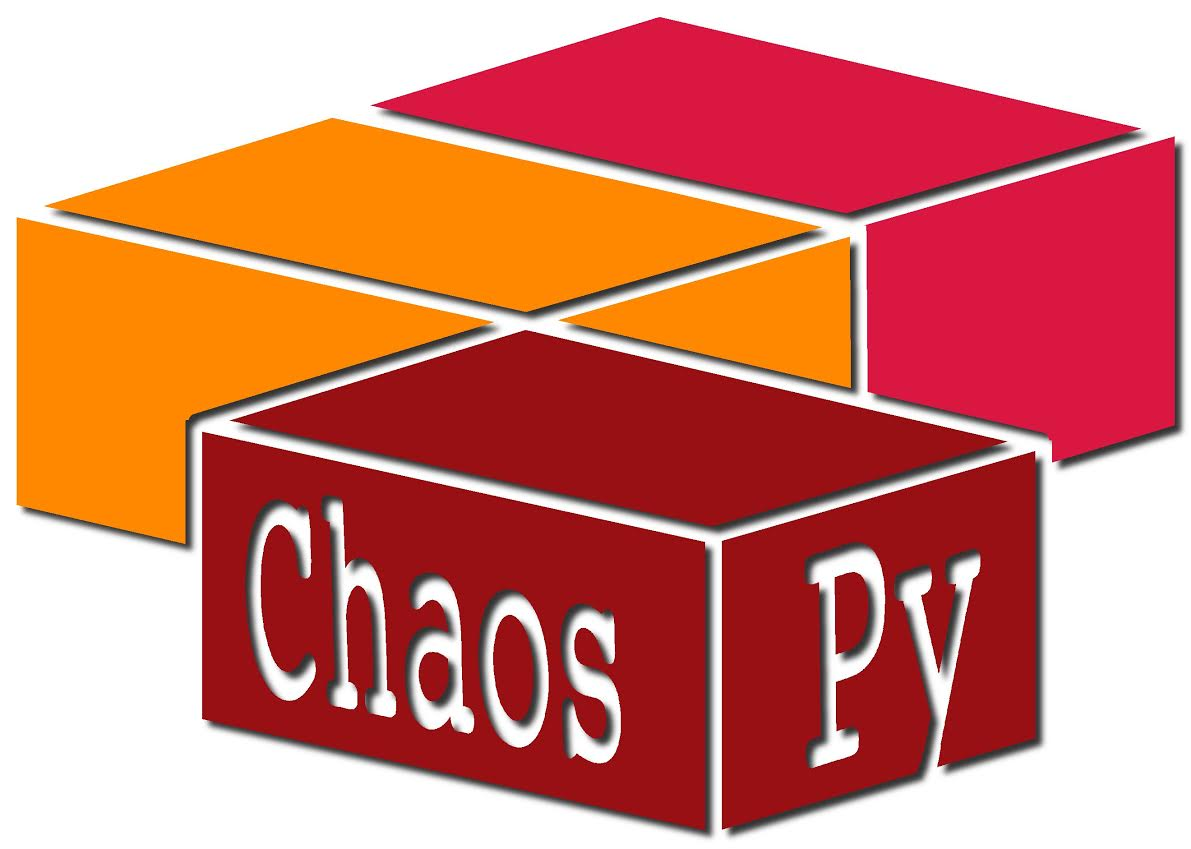
\includegraphics[width=.5\textwidth]{chaospy_logo.jpg}
  \end{center}
  \begin{alert}{Installation instructions:}

%      \href{https://github.com/hplgit/chaospy}{https://github.com/hplgit/chaospy}
\verb;http://github.com/hplgit/chaospy/;
  \end{alert}

    \begin{alert}{Interactive sessions:}

\verb;path/to/ipython/notebook/sessions;
  \end{alert}
\end{frame}

\begin{frame}[fragile]{Practicle application involving bloodflow
    simulations}{}
    \begin{columns}
        \column{.5\textwidth}
        \begin{center}
    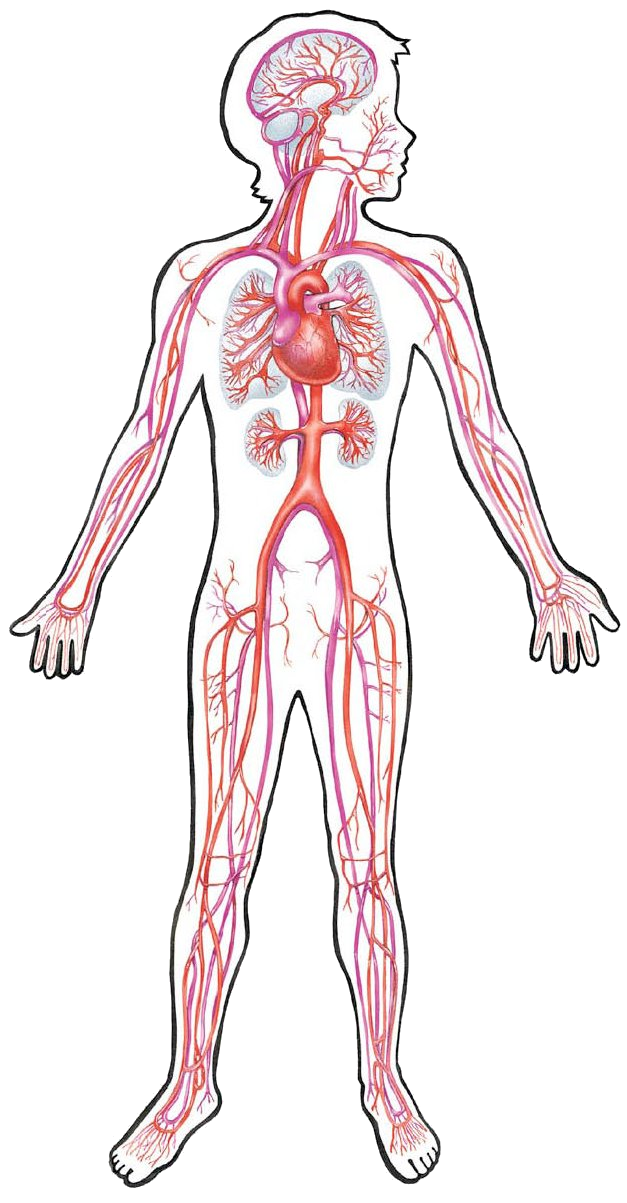
\includegraphics[width=.6\textwidth]{ntnu/arterialHumanPicture.png}
        \end{center}
        \column{.5\textwidth}
        \begin{center}
    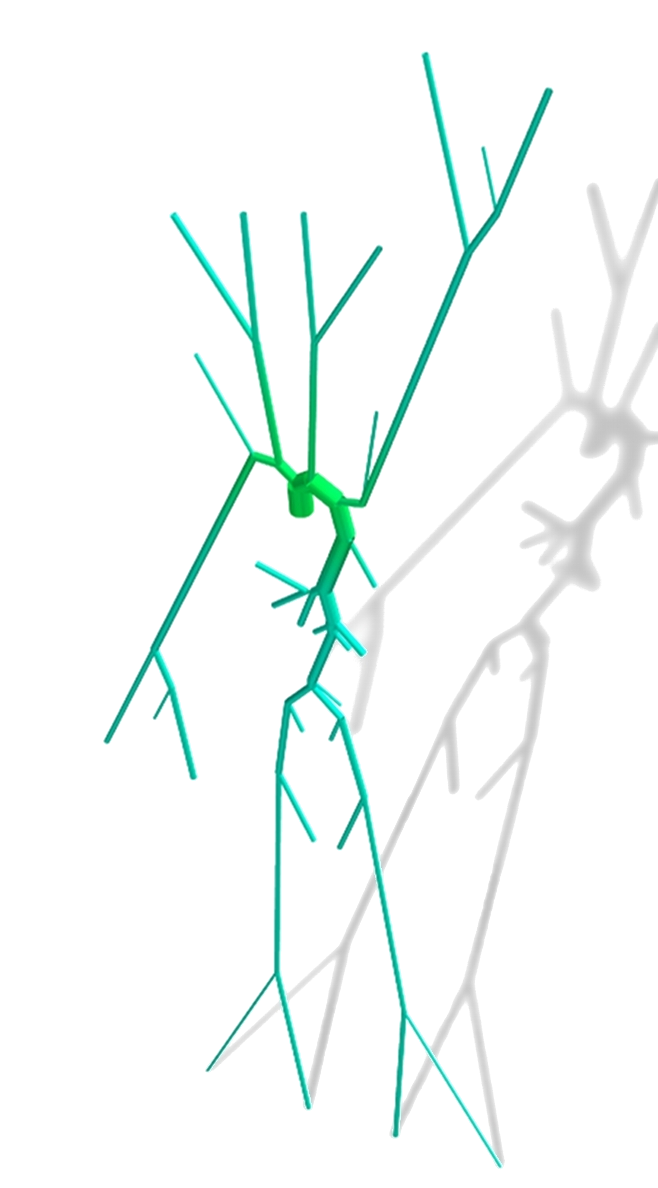
\includegraphics[width=.6\textwidth]{ntnu/arterialTreeMascot3D.png}
        \end{center}
    \end{columns}
    \small
    \begin{flushright}
        In colaboration with V. Eck and L. Hellevik
    \end{flushright}
\end{frame}

\begin{frame}{Modelling require uncertainty quantification}{}
    \begin{columns}
        \column{.3\textwidth}
        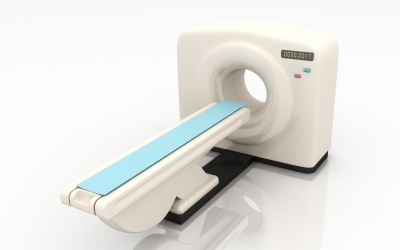
\includegraphics[width=\textwidth]{ntnu/ID-10015904.jpg}
        \column{.3\textwidth}
        
\includegraphics[width=\textwidth]{ntnu/STARFiSh-Logo_small_transparent.png}
        \column{.3\textwidth}
        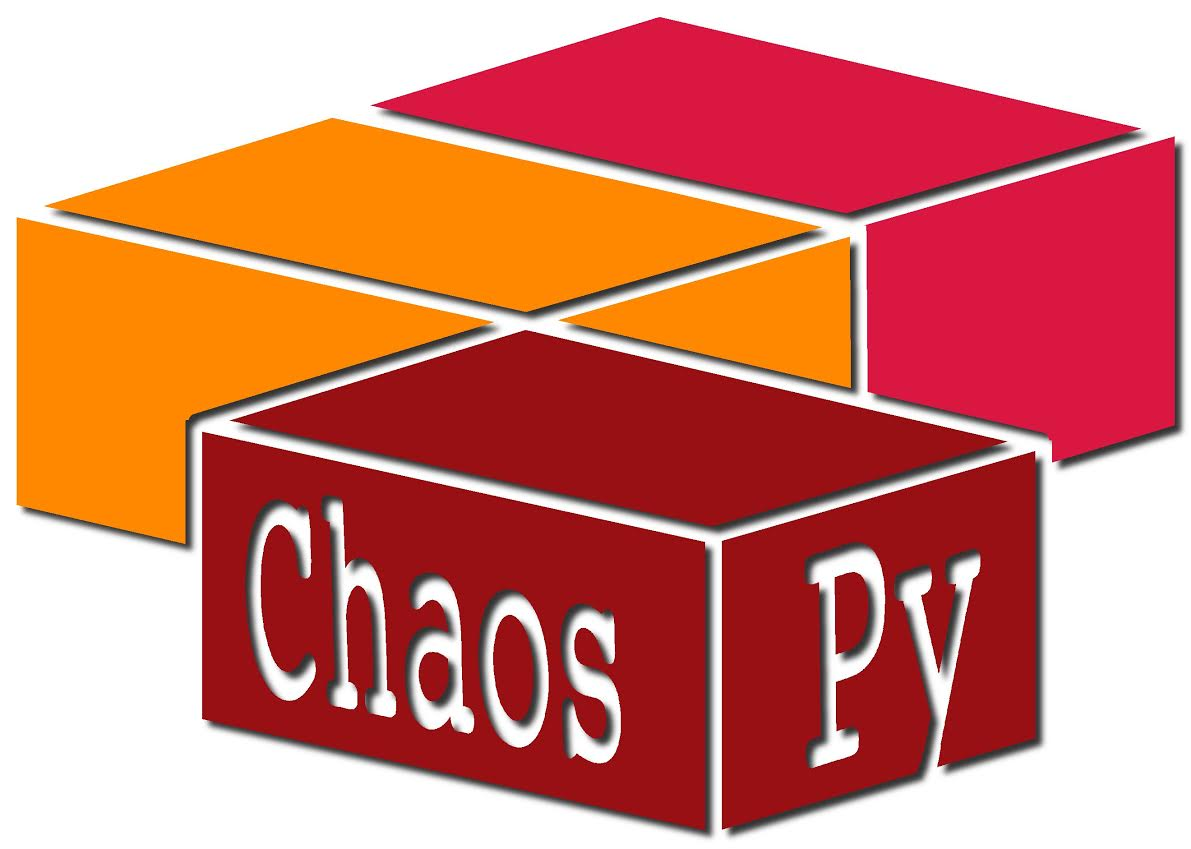
\includegraphics[width=\textwidth]{chaospy_logo.jpg}
    \end{columns} \pause
    \begin{center}
    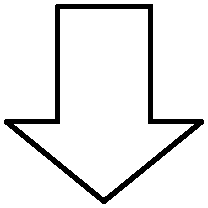
\includegraphics[width=.1\textwidth]{figures/south.pdf}
    \end{center}
    \begin{columns}
        \column{.5\textwidth}
        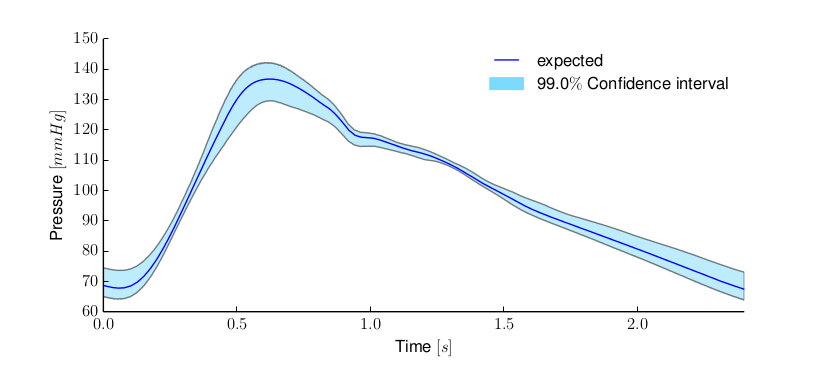
\includegraphics[width=\textwidth]{ntnu/AorticPressure_parameterUncertainty.png}
        \column{.5\textwidth}
        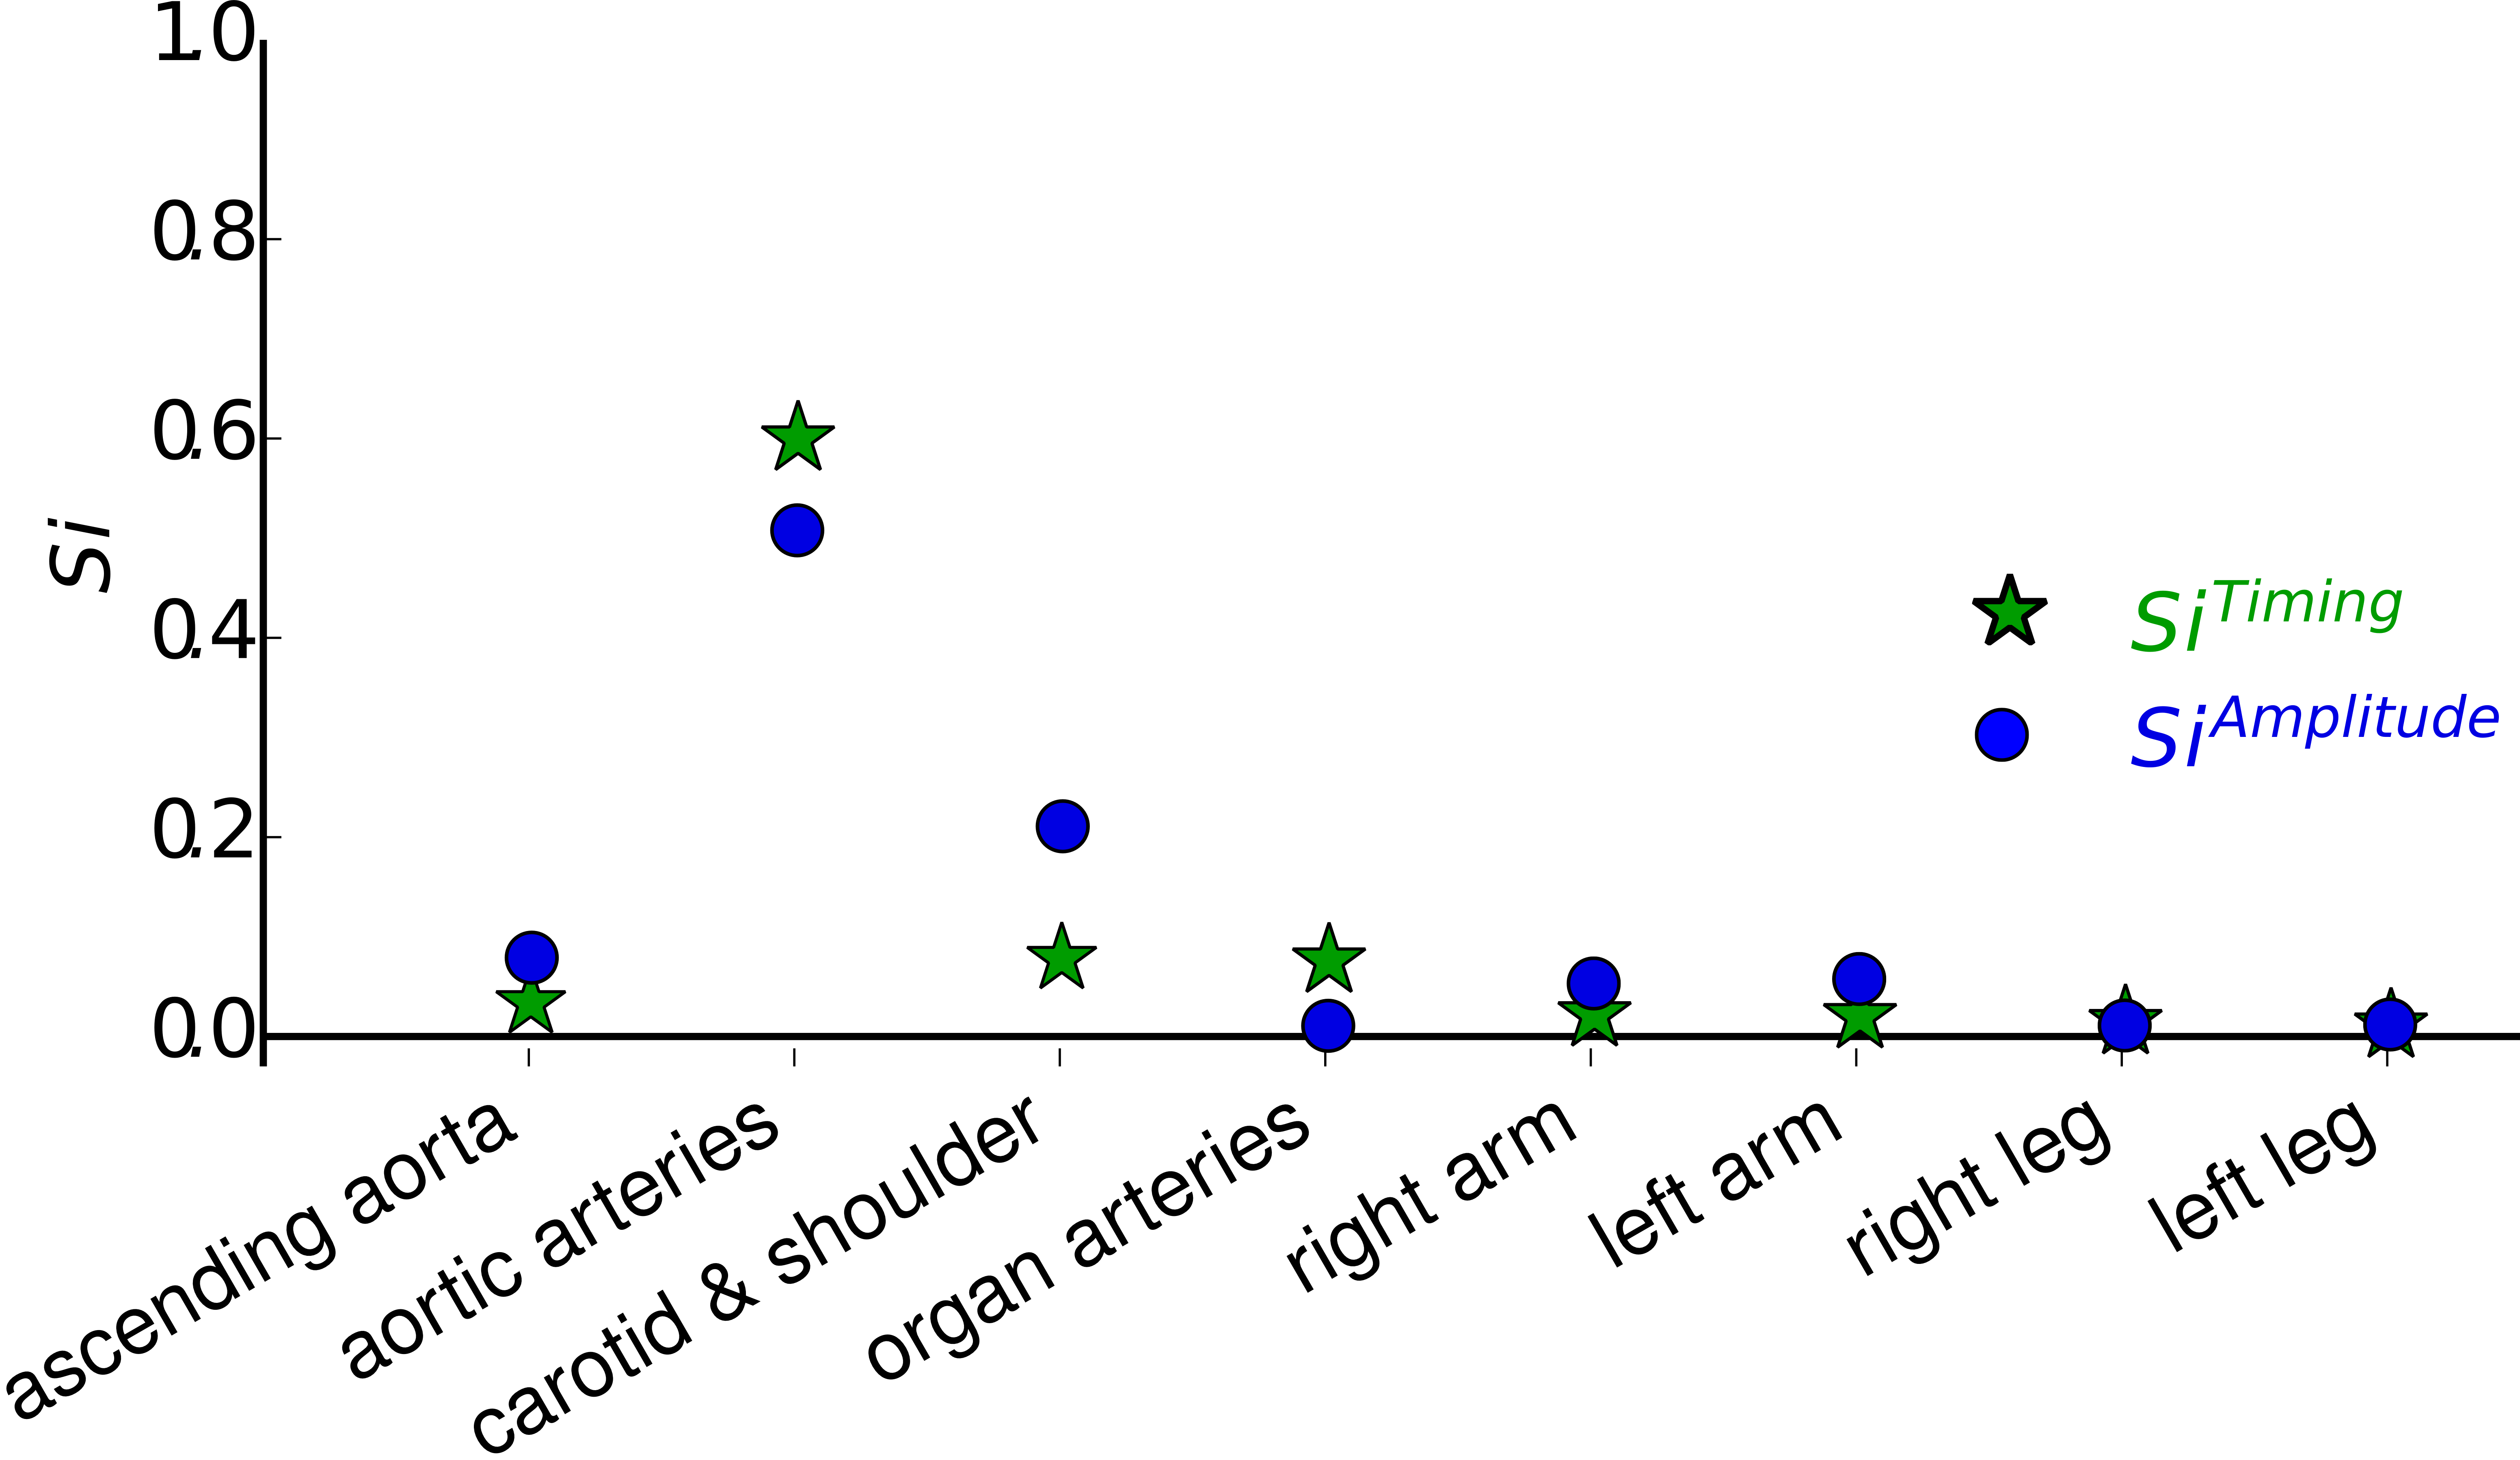
\includegraphics[width=\textwidth]{ntnu/results/sensitivity-pointOfinflection.png}
    \end{columns}
    \end{frame}

\section{Introduction}

\begin{frame}[fragile]
  {Introducing a naive testcase as a working example}
  \pause
  \begin{align*}
    \frac{d u(x)}{dx} & =-au(x) & u(0) &= I
  \end{align*}
  \begin{itemize}
    \item[$u$] The quantity of interest
    \item[$x$] Spatio-temperal locations
    \item[$a,I$] Parameters containting uncertainties
  \end{itemize}
  \pause
  \begin{center}
    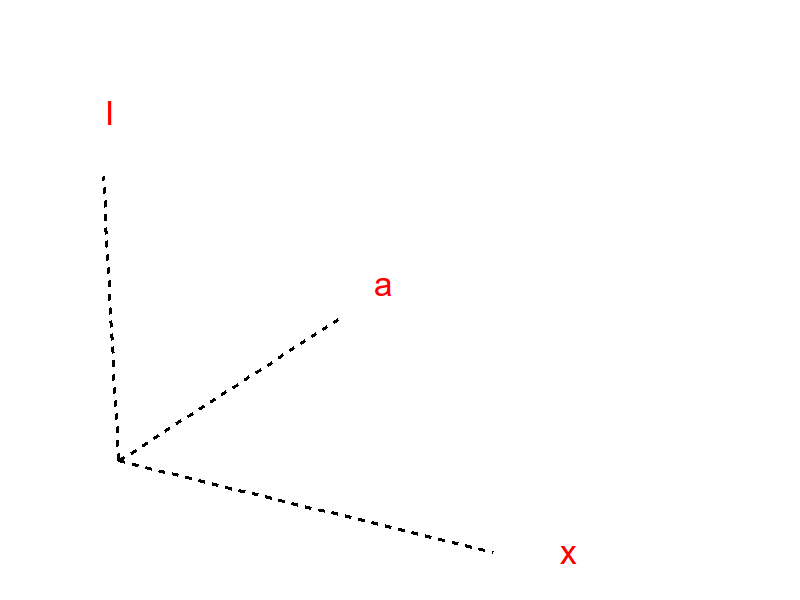
\includegraphics[width=.5\textwidth]{probspace.png}
  \end{center}
\end{frame}



%  \begin{frame}
%   \frametitle{Introducing the problem}
%   We start by looking at the 1D problem:
%   The area if interest is 
%   \[x=[0,10]\]
%  %  We also add the complication
%  %   \[a = \begin{cases}
%  %         a & t<5\\
%  %         2a & t \geq 5
%  %        \end{cases}\]
%  \end{frame}

\begin{frame}
 {Trivial models can be analysed analytically}
 \[
 u(x; a, I) = Ie^{-ax}
 \]
%  \[E(u) = \int_0^{10}\]
\pause
Initially assume model parameters:
\begin{align*}
a &\sim \text{Uniform(0, 0.1)} & I&=1
\end{align*}
\pause
  \begin{align*}
    E(u) &= \int_0^{0.1}e^{-ax}\frac{1}{10}da
    = -\frac{1}{10x}\left(e^{-0.1x}-1\right)
    = \frac{1-   e^{-0.1x}}{10x} \\ 
    \onslide<4->{ Var(u) &= 
    \int_0^{0.1}\left(e^{-ax}\right)^2\frac{1}{10}da - E(u)^2 =
   \frac{1 - e^{-0.2ax}}{20x} - \left(\frac{1-   e^{-0.1x}}{10x}\right)^2}
 \end{align*}
\end{frame}

\begin{frame}[fragile]
{Non-trivial models can be analysed using Monte Carlo
integration}

    \begin{figure}
    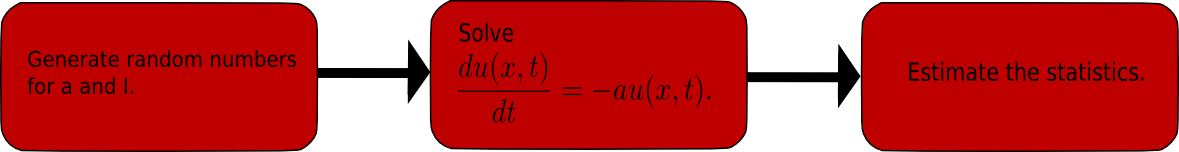
\includegraphics[width=\textwidth]{MC.png}
  \end{figure}
\end{frame}

\begin{chaospy}{Monte Carlo with chaospy}
    \scriptsize
\begin{lstlisting}[language=python]
import chaospy as cp
import numpy as np

def u(x, a):
  return np.exp(-a*x)
    
|\pause|
a = cp.Uniform(0.0.1)
  
samples_a = a.sample(1000)
|\pause|
x = np.linspace(0, 10, 100)
|\pause|
U = [u(x,q) for q in samples_a]
|\pause|
E = np.mean(U)
Var = np.var(U)
\end{lstlisting}
\end{chaospy}

\begin{frame}
  \frametitle{Convergence of Monte Carlo is slow}
  \begin{align*}
  \varepsilon_E &= \int_0^{10}|E(u) - E(\hat{u})|\,dx &
  \varepsilon_{Var} &= \int_0^{10}|Var(u) - Var(\hat{u})|\,dx
  \end{align*}
  \begin{center}
    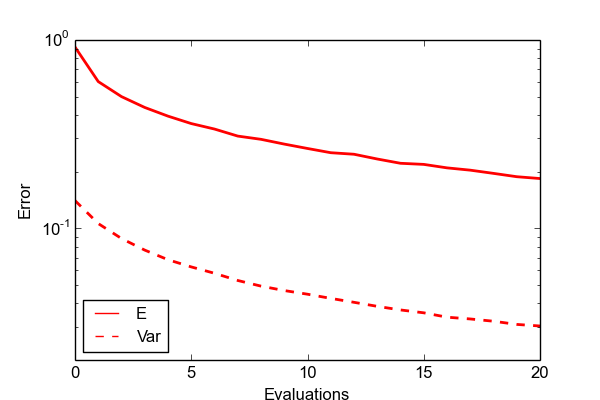
\includegraphics[width=0.75\textwidth]{MC_convergence_1D_1.png}
  \end{center}
\end{frame}



\section{Polynomial Chaos}

\begin{frame}
  \frametitle{Monte Carlo is based on the idea of indirect sampling}
  \begin{center}
   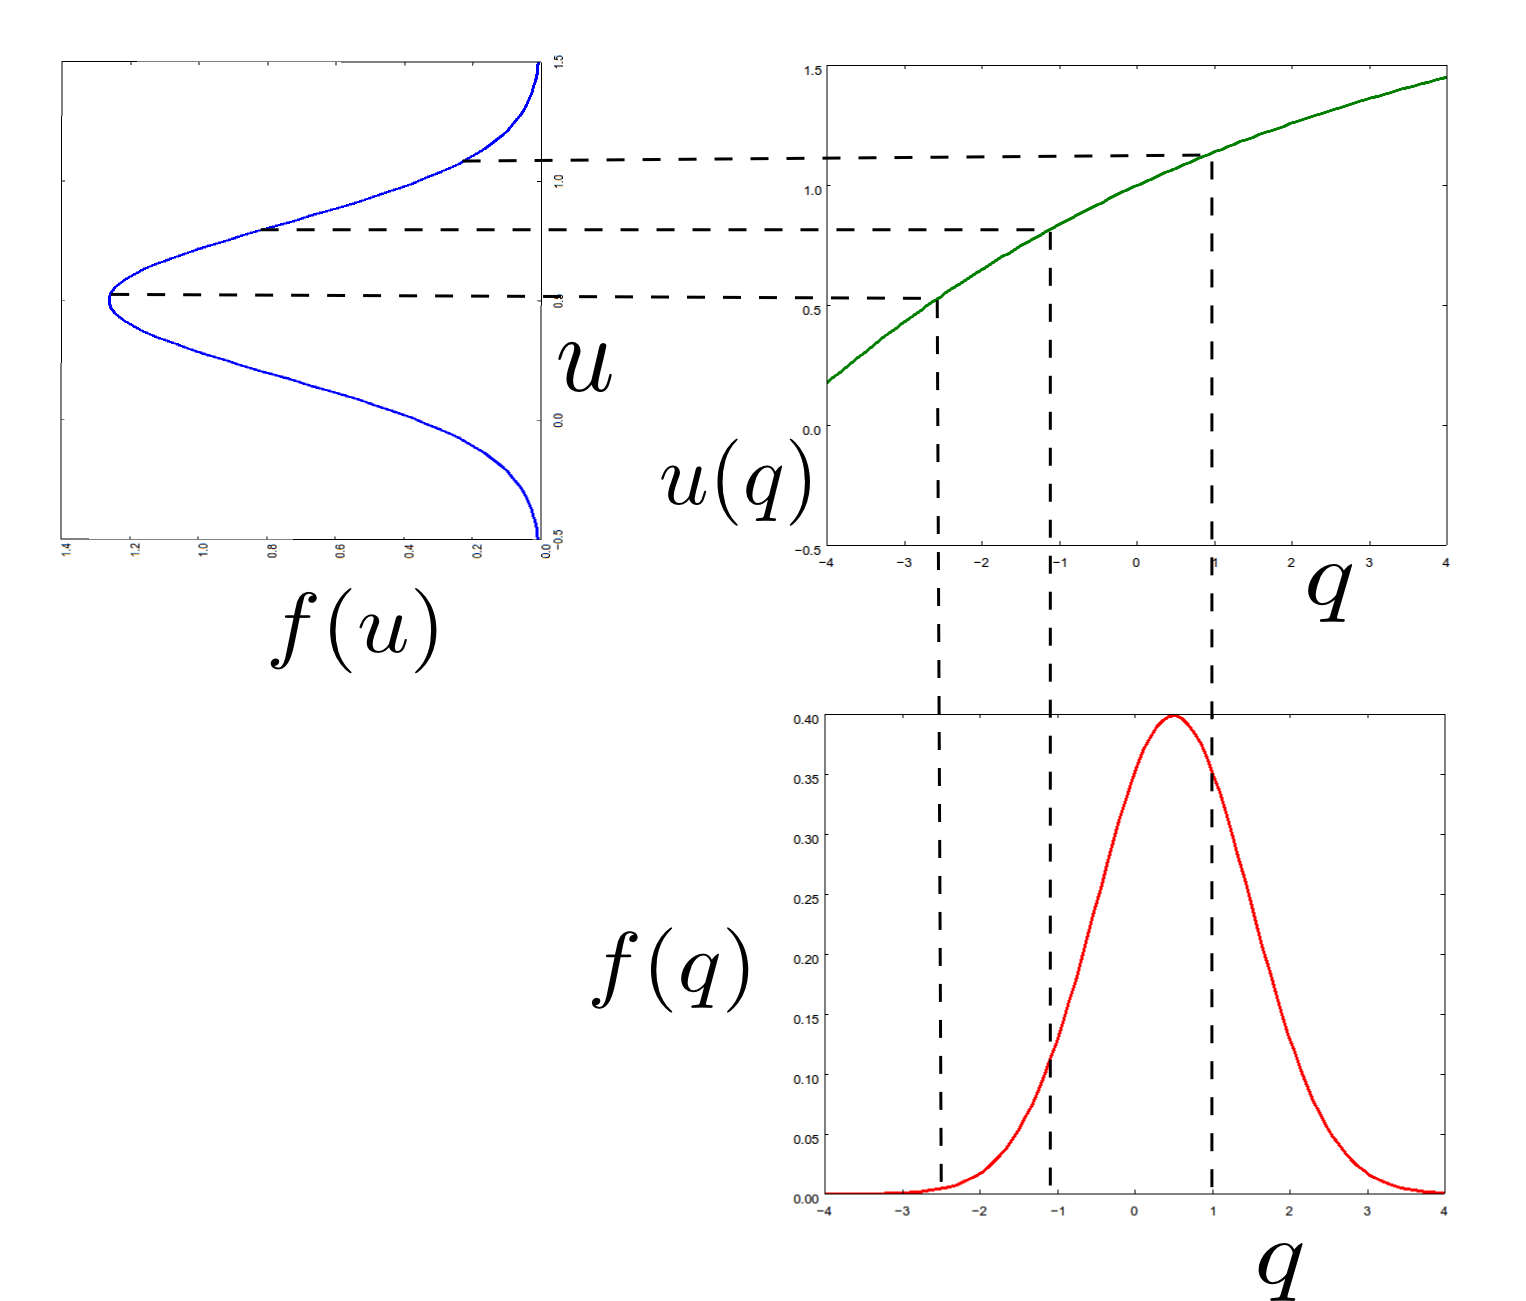
\includegraphics[width=0.8\textwidth]{mapping.png}
  \end{center}
\end{frame}

\begin{frame}[fragile]{Using Lagrange polynomials to approximate the model}{}
    \begin{align*}
        u(x;a) &\approx \hat u_M(x;a) =
        \sum_{n=0}^N c_n(x) P_n(a) & N&=M+1,
    \end{align*}
    where
    \begin{itemize}
        \item[$c_n$] are model evaluations $u(x, a_n)$
        \item[$P_n$] are Lagrange polynomials:
            \begin{align*}
                P_n(a) &= \prod_{\substack{m=0 \\ m\neq n}}^N \frac{a-a_n}{a_m-a_n}
            \end{align*}
        \item[$a_n$] are collocation nodes
    \end{itemize}
\end{frame}

\begin{frame}
  \frametitle{Much better convergence properties than Monte Carlo}
  \begin{center}
    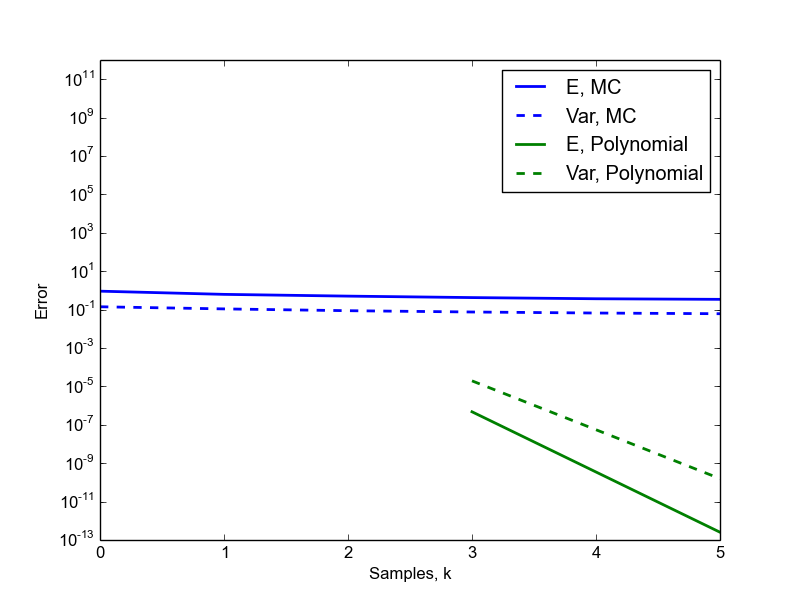
\includegraphics[width=0.8\textwidth]{MC_convergence_1D_2_short.png}
  \end{center}
\end{frame}

\begin{frame}
  \frametitle{Stochastic analysis of model approximations can be
  dangerous}
  \begin{center}
    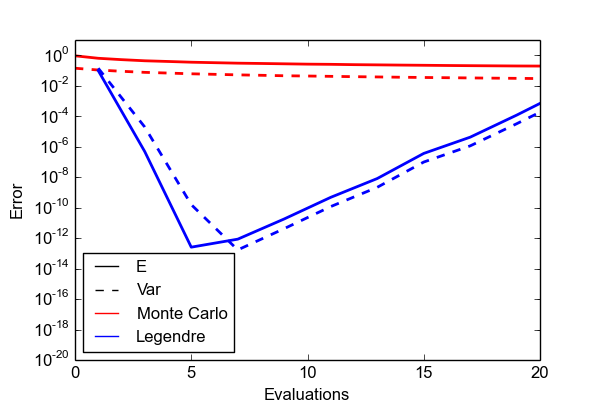
\includegraphics[width=0.8\textwidth]{MC_convergence_1D_2.png}
  \end{center}
\end{frame}



\begin{frame}
  \frametitle{Combining polynomial approximation with uncertainty
  quantification well requires a better underlying theory}

    \begin{align*}
        \inner{u,v} &= E(u\cdot v) \qquad
        \norm{u} = \sqrt{\inner{u,u}} \\
    \uncover<2->{&= \int f_Q(q)u(x,q)v(x,q)dq}
  \end{align*}
  where $Q$ is a random vector, i.e. $(a,I)$.
  \pause\pause\newline

  \begin{alert}
      {Orthogonality:}
  \[\langle P_n,P_m\rangle =
  \begin{cases}
    \norm{P_n}^2 & n = m \\
    0 & n \neq m
  \end{cases}\]
  \end{alert}

\end{frame}

\begin{frame}{Coefficients are Fourier when polynomials are
    orthogonal}{}
    \begin{align*}
        u &= \sum_{n=0}^N c_n P_n \\
        \onslide<2->{\inner{u,P_k} &=
        \inner{\sum_{n=0}^N c_n P_n,P_k}}
        & \onslide<2>{k&=0,\dots,N} \\
        \onslide<3->{&=
        \sum_{n=0}^N c_n \inner{P_n,P_k}}
        & \onslide<3>{k&=0,\dots,N} \\
        \onslide<4->{&=
        c_k \inner{P_k,P_k}}
        & \onslide<4>{k&=0,\dots,N} \\ \\
        \onslide<5>{
        c_k &= \coef{u}{P_k} &
        k&=0,\dots,N}
    \end{align*}
\end{frame}

\begin{frame}{Optimality linked to statistical property}{}
    \begin{align*}
        (c_0,\dots,c_N)
        &= \argmin_{c_0,\dots,c_N} \norm{u-\hat u_M} \\\\
        \onslide<2->{
        &= \argmin_{c_0,\dots,c_N} \norm{u-\hat u_M}^2 \\\\
        }
        \onslide<3->{
        &= \argmin_{c_0,\dots,c_N} \E{(u-\hat u_M)^2} \\\\
        }
        \onslide<4->{
        &= \argmin_{c_0,\dots,c_N} \Var{u-\hat u_M} \\\\
        }
    \end{align*}
\end{frame}

\begin{frame}{The mean and variance has a simpler form}{}
    \pause
    \begin{alert}{Assumption:}
        $P_0 = 1$
    \end{alert}
    \begin{align*}
        \onslide<3->{\E{\hat u_M} &=
        \E{\sum_{n=0}^N c_n P_n}}
        &
        \onslide<7->{\Var{\hat u_M} &=
        \Var{\sum_{n=0}^N c_n P_n}}
        \\
        \onslide<4->{&=
        \sum_{n=0}^N c_n \E{P_n}}
        &
        \onslide<8->{&=
        \sum_{\substack{n=0\\m=0}}^N c_n c_m
        \left(\E{\!P_nP_m\!}\!-\!\E{\!P_n\!}\!\E{\!P_m\!}\right)}
        \\
        \onslide<5->{&=
        \sum_{n=0}^N c_n \inner{P_n, P_0}}
        &
        \onslide<9->{&=
        \sum_{\substack{n=0\\m=0}}^N c_nc_m\inner{P_n,P_m}-c_0^2}
        \\
        \onslide<6->{\E{\hat u_M}&=c_0}
        &
        \onslide<10->{\Var{\hat u_M}&=
        \sum_{n=1}^N c_n^2\norm{P_n}}
    \end{align*}
\end{frame}

\begin{frame}
 \frametitle{Construct an orthogonal polynomial expansion using
 Gram-Schmidt orthogonalization}
%  Assumption: We are in 1D and have $a +~ F_q$ and $I = 1$. 
 \[v_0, v_1,...,v_N = 1, q,...,q^N\]
 \pause
 The Gram Schmidt method is
 
 \begin{align*}
    P_0 &= v_0\\
    \uncover<3-> {P_n &= v_n - \sum_{m=0}^{n-1} \frac{\inner{v_n,P_m}}{\norm{P_m}^2}}\\
    \uncover<4-> {&= v_n -
    \sum_{m=0}^{n-1}\frac{\E{v_nP_m}}{\E{P_m^2}}}
 \end{align*}

\end{frame}

\begin{chaospy}{Gram-Schmidt with chaospy}
\begin{lstlisting}[language=python]
M = 5; D = 1; N = M - 1

a = cp.Uniform(0,0.1)
|\pause|
v = cp.basis(0,M,1)
P = [v[0]]
|\pause|
for n in xrange(1,N):
    p = v[n]
    for m in xrange(0,n):
        p -= P[m]*cp.E(v[n]*P[m],a)
                            /cp.E(P[m]**2,a)
    P.append(p)
P = cp.Poly(P)
 \end{lstlisting}
\end{chaospy}


\begin{frame}
 \frametitle{Plot of all generated polynomials}
  \begin{figure}
    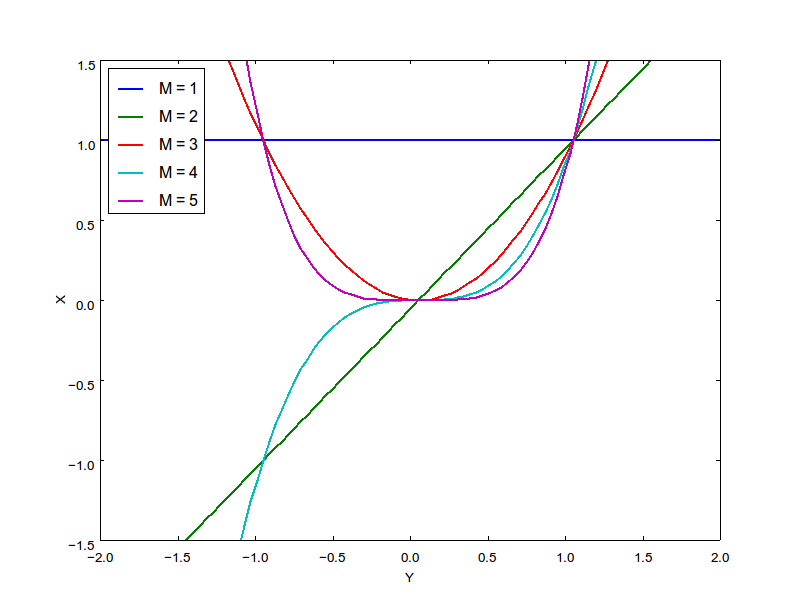
\includegraphics[width=0.85\textwidth]{gramschmidtpoly.png}
  \end{figure}
\end{frame}


\begin{frame}
 \frametitle{Most constructors of orthogonal polynomials are
 illposed}
  % TODO
  % high: formula for error
%   \[\varepsilon_E = \int_0^{10}|E(u) - E(\hat{u})|\,dx\]
     \begin{figure}
    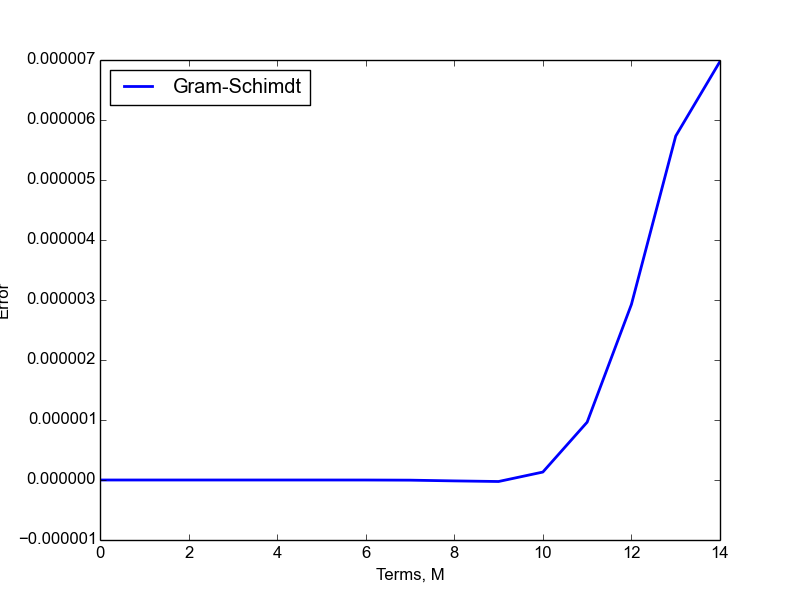
\includegraphics[width=0.85\textwidth]{gramschmidterror1.png}
  \end{figure}
  
 \end{frame}


\begin{frame}
 {The only numerically stable method for
 calculating orthogonal polynomials is through the discretized
 Stiltjes method}
 \pause
 Three terms recursion relation:
 \begin{align*}
     P_{n+1} &= (x-A_n) P_n - B_n P_{n-1} &
     P_{-1} &= 0 & P_0 &= 1,
 \end{align*}
    \pause
   where
   \begin{align*}
   A_n &= \frac{\langle qP_n,P_n\rangle_Q}{\norm{P_n}^2}
   &
  B_n &= 
  \begin{cases}
  \frac{\norm{P_n}^2}{\norm{P_{n-1}}^2} & n > 0\\
  \norm{P_n}^2 & n = 0
  \end{cases}
   \end{align*}
  \end{frame}

  
  
\begin{frame}
 \frametitle{Askey scheme, organization of orthogonal polynomials}
 The askey scheme gives a relation between a probability distribution and the corresponding orhogonal polynomial.
 \begin{center}
  \begin{tabular}{lll}
 Distribution & Polynomial & Support \\\hline
  Gaussian & Hermite & $(-\infty, \infty)$ \\
  Gamma & Laguerre & $[0,\infty]$ \\
  Beta & Jacobi & $[a,b]$ \\
  Uniform & Legendre & $[a,b]$ \\\hline
   \end{tabular}
\end{center}  
 \end{frame}  
  
  
\begin{chaospy}{
    Three terms recursion in Chaospy}
\begin{lstlisting}[language=python]
import chaospy as cp

M = 3
a = cp.Normal()
P = cp.orth_ttr(M, a)

print P

[1.0, q0, q0^2-1.0, q0^3-3.0q0]
\end{lstlisting}
\end{chaospy}

\begin{frame}
 \frametitle{Discretized Stiltjes method is numerically stable}
    % TODO
    % high: error-formula
    % med: trunkation
%  \begin{align*}
%   \varepsilon_E &= \int_0^{10}|E(u) - E(\hat{u})|\,dx &
%   \end{align*}
 
    \begin{figure}
    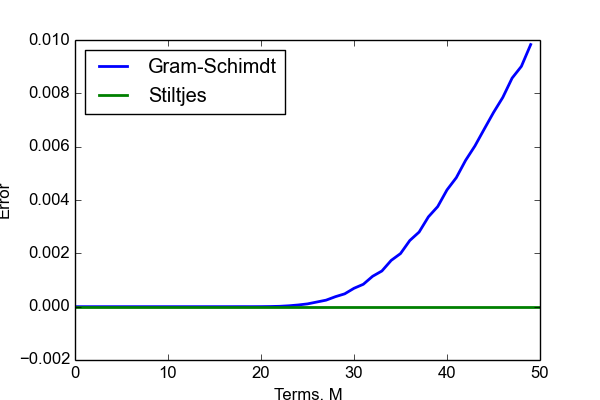
\includegraphics[width=0.85\textwidth]{gramschmidterror2.png}
  \end{figure} 
 \end{frame}
  

%  \begin{chaospy}{Finding the Fourier coefficients}
%   \begin{lstlisting}[language=python]
%  def u(x,a):
%    ax = np.outer(a,x)
%    return np.exp(-ax)
%  |\pause|
%  m = 2
%  a = cp.Uniform(0,0.1)
%  x = np.linspace(0, 10, 100)
%  |\pause|
%  P, norm = cp.orth_ttr(m, a, retall=True)|\pause|
%  nodes, weights = cp.generate_quadrature(m+1, a,
%                                          rule="G")|\pause|
%  solves = u(x,nodes[0])|\pause|
%  u_hat, c = cp.fit_quadrature(P, nodes, weights,
%                               solves,retall=True)
%  \end{lstlisting}
%  
%  \end{chaospy}
\begin{frame}
 {Repetition of the problem}
 \[  u(x; a, I) = Ie^{-ax}\]
\pause
Initially assume model parameters:
\begin{align*}
a &\sim \text{Uniform(0, 0.1)} & I&=1
\end{align*}
\pause
\begin{align*}
    E(u) &= \frac{1-e^{-0.1x}}{10x} & Var(u) &=
   \frac{1 - e^{-0.2ax}}{20x} - \left(\frac{1-   e^{-0.1x}}{10x}\right)^2
 \end{align*}
 \pause
   \begin{align*}
  \varepsilon_E &= \int_0^{10}|E(u) - E(\hat{u})|\,dx &
  \varepsilon_{Var} &= \int_0^{10}|Var(u) - Var(\hat{u})|\,dx
  \end{align*}
\end{frame}

\begin{frame}
\frametitle{Convergence of orthogonal polynomial approximation}

    % TODO
    % med: truncation
  \begin{figure}
    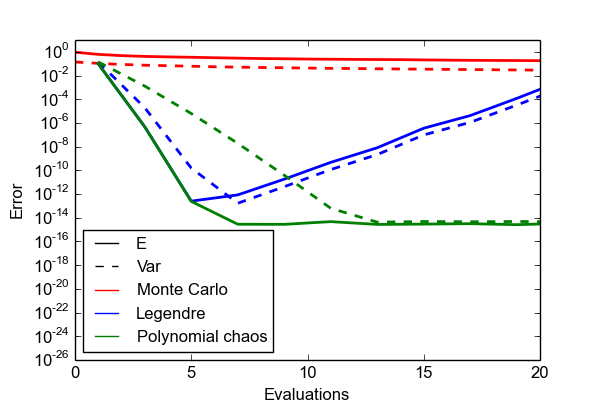
\includegraphics[width=0.8\textwidth]{MC_convergence_1D_3.png}
  \end{figure}
   \end{frame}


\begin{frame}
 \frametitle{Extending the theory to multiple dimensions}
 \pause
  \begin{align*}
  P_n &= P^{(1)}_n, ..., P^{(D)}_{n_D}
  & n\longleftrightarrow (n_1, ..., n_D)
  \end{align*}
  \pause
  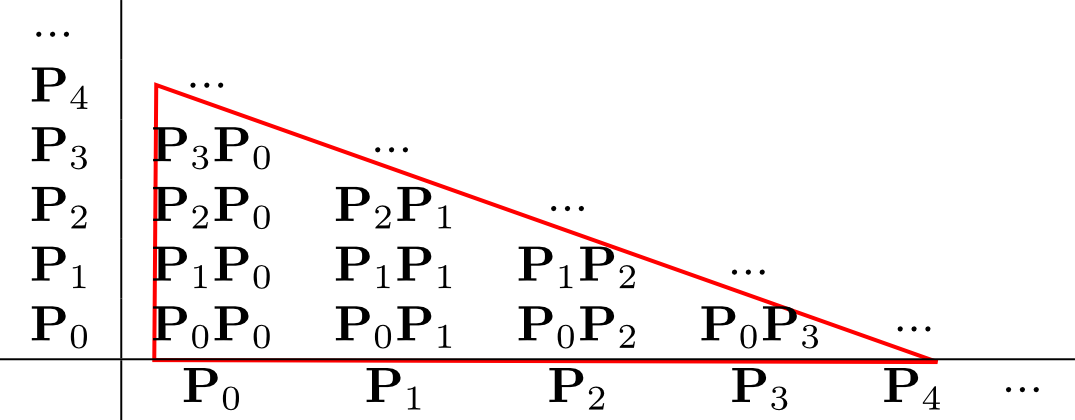
\includegraphics[width=\textwidth]{multidim.png}
   
 % \begin{tabular}{l|cccccc}
 % ... &&&&&\\ 
  % $\mathbf{P}_{4}$& ...&&&& \\
 %   $\mathbf{P}_{3}$ &	$\mathbf{P}_{3}\mathbf{P}_{0}$ & ... && &\\
 %   $\mathbf{P}_{2}$ &	$\mathbf{P}_{2}\mathbf{P}_{0}$ & $\mathbf{P}_{2}\mathbf{P}_{1}$ & ... &&& \\
 %   $\mathbf{P}_{1}$ &	$\mathbf{P}_{1}\mathbf{P}_{0}$ &$\mathbf{P}_{1}\mathbf{P}_{1}$& $\mathbf{P}_{1}\mathbf{P}_{2}$ & ...&&\\
 %   $\mathbf{P}_{0}$ &	$\mathbf{P}_{0}\mathbf{P}_{0}$ &$\mathbf{P}_{0}\mathbf{P}_{1}$& $\mathbf{P}_{0}\mathbf{P}_{2}$ & $\mathbf{P}_{0}\mathbf{P}_{3}$ & ...\\ \hline
%		     &	$\mathbf{P}_{0}$	&$\mathbf{P}_{1}$& $\mathbf{P}_{2}$ & $\mathbf{P}_{3}$ & $\mathbf{P}_{4}$& ...
%  \end{tabular}
 \end{frame}


\begin{frame}
  \frametitle{Construct polynomial approximation}
  \begin{columns}[c] 
    \column{.5\textwidth}
    \begin{center}
      Multi-index\\
    \begin{tabular}{c}
    \\
      $\mathbf{P}_{00}$\\
    $\mathbf{P}_{10} \quad \mathbf{P}_{01}$\\
    $\mathbf{P}_{20} \quad \mathbf{P}_{11}\quad \mathbf{P}_{02}$\\
    $\mathbf{P}_{30} \quad \mathbf{P}_{21}\quad \mathbf{P}_{12}\quad ...$ 
  \end{tabular}
    \end{center}

\column{.5\textwidth}

\begin{center}
Single-index\\
\begin{tabular}{c}
\\
    $\mathbf{P}_{0}$\\
    $\mathbf{P}_{1} \quad \mathbf{P}_{2}$\\
    $\mathbf{P}_{3} \quad \mathbf{P}_{4}\quad \mathbf{P}_{5}$\\
    $\mathbf{P}_{6} \quad \mathbf{P}_{7}\quad \mathbf{P}_{8}\quad ...$ 
  \end{tabular}
\end{center}
  \end{columns}
\end{frame}


\begin{frame}
 \frametitle{Orthogonality for multivariate polynomials}
\begin{align*}
    \inner{ \bm P_n, \bm P_m} &= \E{P_{n_1}^{(1)}\cdots P_{n_D}^{(D)}\cdot
    P_{m_1}^{(1)}\cdots P_{m_D}^{(D)}}\\\\
    \onslide<2-> {&= \E{P_{n_1}^{(1)}\cdot P_{m_1}^{(1)}}\cdots
  \E{P_{n_D}^{(D)}\cdot P_{m_D}^{(D)}}} \\\\
  \onslide<3-> {&= \inner{ P_{n_1}^{(1)}\cdot P_{m_1}^{(1)} }\cdots
  \inner{ P_{n_D}^{(D)}\cdot P_{m_D}^{(D)} }} \\\\
  \onslide<4-> {&=
  \norm{P_{n_1}^{(1)}}\delta_{n_1m_1}\cdots\norm{P_{n_D}^{(D)}}\delta_{n_Dm_D}}
  \\\\
  \onslide<5-> {\inner{ \bm P_n, \bm P_m}&=
  \norm{\bm P_n} \delta_{nm}}
\end{align*}

\end{frame}


 \begin{chaospy}{Creating multivariate orthogonal polynomials in Chaospy}
\begin{lstlisting}[language=python]
a = cp.Uniform(0, 0.1)
I = cp.Uniform(8, 10)
dist = cp.J(a,I)
|\pause|
P = cp.orth_ttr(1, dist)
print P
[1.0, q1-9.0, q0]
|\pause|
P = cp.orth_ttr(3, dist)
print cp.E(P[1]*P[2],dist)
0.0 |\pause|
print cp.E(P[3]*P[3],dist)
0.0888888888903
\end{lstlisting}
\end{chaospy}
 
 
 \begin{frame}
 {The multidimensional problrm }
 \[  u(x; a, I) = Ie^{-ax}\]
\pause
Initially assume model parameters:
\begin{align*}
a &\sim \text{Uniform(0, 0.1)} & I&= \text{Uniform(8, 10)}
\end{align*}
 \pause
   \begin{align*}
  \varepsilon_E &= \int_0^{10}|E(u) - E(\hat{u})|\,dx &
  \varepsilon_{Var} &= \int_0^{10}|Var(u) - Var(\hat{u})|\,dx
  \end{align*}
\end{frame}
 
 
\begin{frame}
 \frametitle{Convergence of a multidimensional problem}
 % TODO
 % high: error formulae
%   \begin{align*}
%   \varepsilon_E &= \int_0^{10}|E(u) - E(\hat{u})|\,dx &
%   \varepsilon_{Var} &= \int_0^{10}|Var(u) - Var(\hat{u})|\,dx
%   \end{align*}
 
\begin{figure}
    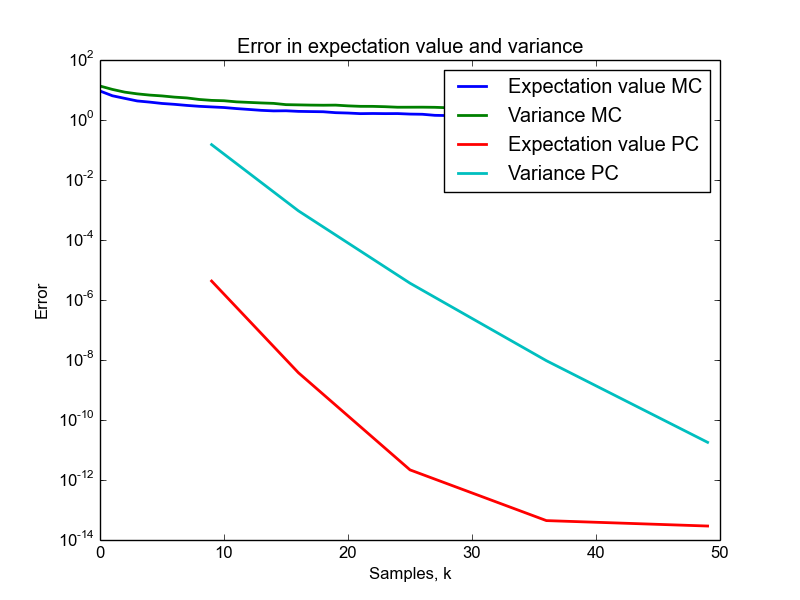
\includegraphics[width=0.85\textwidth]{MC_convergence_2D.png}
  \end{figure}

 \end{frame}

 
 \begin{chaospy}{Teaser of the full implementation}
     \scriptsize
 \begin{lstlisting}[language=python]
def u(x,a, I):
  return I*np.exp(-a*x)
|\pause| 
a = cp.Uniform(0, 0.1)
I = cp.Uniform(8, 10)
dist = cp.J(a,I)|\pause|
|\pause| 
P = cp.orth_ttr(2, dist)
|\pause|
nodes, weights = \
    cp.generate_quadrature(3, dist, rule="G")

x = np.linspace(0, 10, 100)
solves = [u(x, *node) for node in nodes.T]

u_hat = cp.fit_quadrature(P, nodes, weights, solves)

mean, var = cp.E(u_hat, dist), cp.Var(u_hat, dist)
 \end{lstlisting}
\end{chaospy}


\begin{frame}
  \frametitle{The curse of dimensionality}
  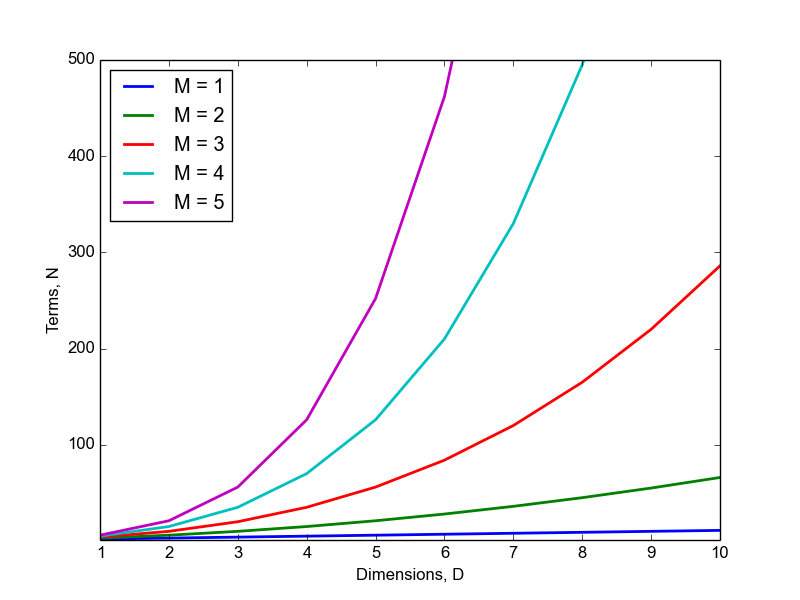
\includegraphics[height = 0.85\textheight]{dimensionality.png}

\end{frame}


\begin{frame}
  \frametitle{Gibb's Phenomena, discontinues methods are troublesome}
  \begin{figure}
  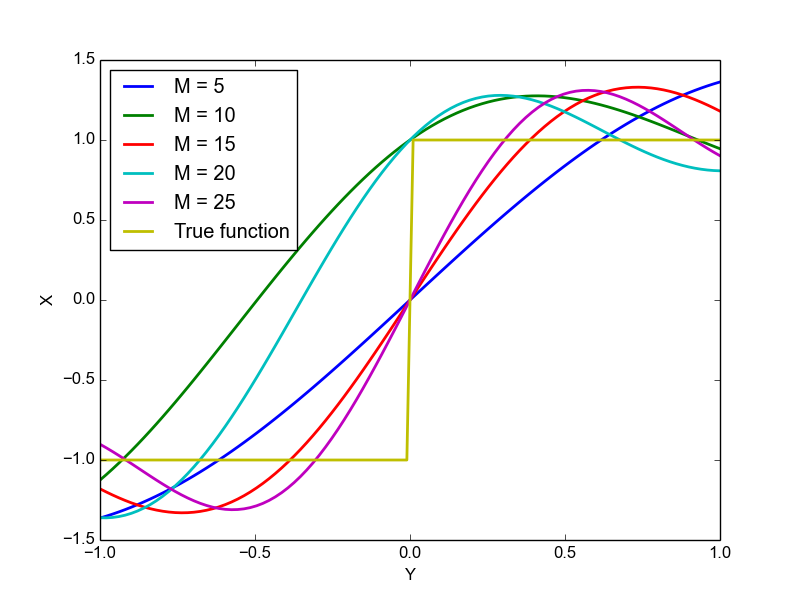
\includegraphics[width=0.85\textwidth]{gibbs.png}
  \end{figure}
  \end{frame}

\begin{frame}
 \frametitle{Higher number of samples justifies higher number of
 collocation nodes}
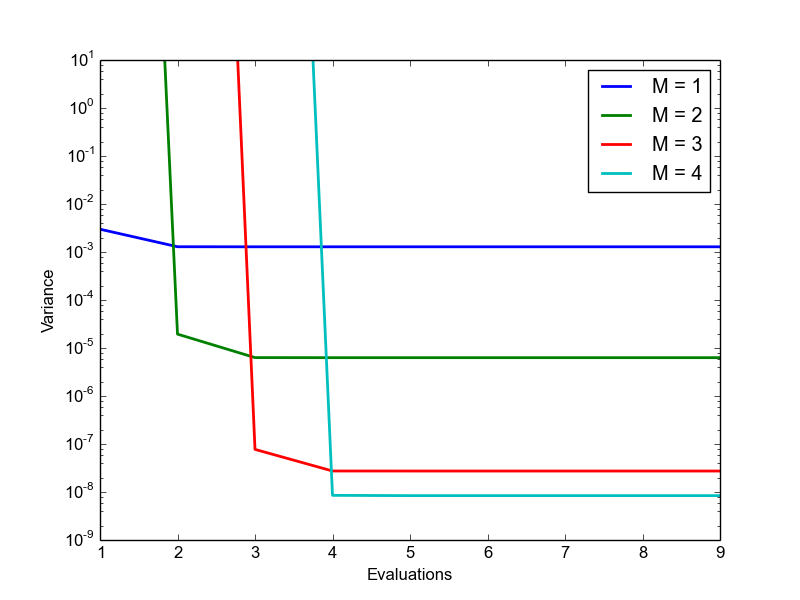
\includegraphics[width=0.9\textwidth]{k_convergence.png}
 \end{frame}


%\begin{frame}
%  \frametitle{What happens if we choose the wrong distribution}
  
%\end{frame}


\end{document}
